\chapter{État de l'art}\label{chap:etat_art}

	La première partie de mon travail a consisté à réaliser un état de l'art sur
	les systèmes Blockchain. Le plan de ce chapitre suivra la chronologie de mes
	recherches. J'ai commencé par approfondir mes connaissances sur le
	fonctionnement général des Blockchains~\cite{bitcoin}, avant de
	m'intéresser aux modèles utilisés pour décrire l'évolution de tels systèmes
	(\cite{static_backbone} et \cite{dynamic_backbone}). J'ai ensuite étudié un
	algorithme de compression dans un modèle dit \textit{statique}~\cite{mls}.
	Enfin, j'ai étudié le travail déjà effectué par l'équipe avant mon arrivée.
	L'objectif de ce travail étant d'adapter l'algorithme de compression à un
	modèle \textit{dynamique}, plus proche de la réalité.

	En plus de la lecture approfondie des articles auxquels je fais référence,
	j'ai refait de nombreuses preuves et calculs des travaux présentés dans les
	sections \ref{sec:dynamic} et \ref{sec:mls}. Cela m'a permis de me
	familiariser avec les outils et les concepts qui allaient m'être nécessaires
	pour la suite de mon travail de recherche.

    J'ai pris la liberté de renommer certaines variables et notations présentes
    dans les articles, afin d'homogénéiser les notations entre elles, et de
    rendre ma présentation plus claire. Une liste des notations relatives à
    chaque section est disponible en annexe~\ref{chap:notations}.
    

\section{Les systèmes Blockchain}\label{sec:blockchain}

    Ma première lecture a été évidemment le livre blanc de Satoshi
    Nakamoto~\cite{bitcoin}. Ce document est la première publication sur le
    sujet et reste une référence incontournable. La Blockchain y est décrite
    comme une solution de paiement décentralisée, sans tiers de confiance. La
    sécurité  du système y est assurée par un historique partagé de toutes les
    transactions. Il est ainsi auditable par tous les participants. La sécurité
    de l'historique est assurée par un mécanisme de preuve de travail (abrégée
    PoW pour Proof Of Work), qui garantit son intégrité.

    Quand un utilisateur (Bob) de la Blockchain veut effectuer un paiement
    auprès d'un autre utilisateur (Alice), il crée une transaction. Bob signe
    cette transaction avec sa clé privée, puis la diffuse sur le réseau. Les
    autres participants peuvent ainsi vérifier que Bob est bien en capacité de
    dépenser les fonds qu'il veut envoyer, et qu'il ne se dédit pas. Pour cela,
    ils vérifient la signature de Bob, et qu'il n'a pas déjà dépensé ces fonds.
     
    La transaction est ensuite ajoutée à l'historique des transactions. Pour
    savoir si Bob est en capacité d'utiliser son argent, on parcourt
    l'historique des transactions en partant de la création de la Blockchain. On
    cherche alors toutes les transactions qui lui sont destinées, mais qu'il n'a
    pas encore dépensées. On appelle ces transactions des UTXOs. Bob peut alors
    présenter ces UTXOs pour prouver qu'il est en capacité de dépenser ces
    fonds.

    D'une manière générale, une Blockchain est une structure de données. Au
    cours de mon travail, je n'ai pas eu besoin de m'intéresser aux données
    stockées, mais uniquement à la structure de la Blockchain. C'est pourquoi
    dans le reste de ce mémoire, je parlerai de données applicatives, sans
    préciser leur nature.


    \subsection{Structure de la chaîne}\label{subsec:fonctionnement}
    
    % Structure de la Blockchain
    Chaque changement d'état des données applicatives est stocké dans des blocs.
    Chaque nœud de la Blockchain stocke une copie de la chaîne de blocs. Quand
    un nœud reçoit un changement des données applicatives, il stocke ce
    changement dans un bloc à la fin de sa chaîne. Il diffuse ensuite ce bloc
    sur le réseau. Les autres nœuds vérifient la validité du bloc, puis
    l'ajoutent à leur chaîne. La chaîne la plus difficile à créer est considérée
    comme la chaîne de référence. Chaque nœud du système peut posséder une
    chaîne légèrement différente des autres. En effet le réseau subit un temps
    de propagation. Un bloc en fin de chaîne peut donc se faire invalider par
    une autre chaîne ayant demandé plus de travail. Cette chaîne n'aurait pas
    encore été reçue par notre nœud initial. Les derniers blocs d'une chaîne
    sont donc instables. Malgré cette instabilité des derniers blocs, chaque
    chaîne du réseau possède un préfixe commun immuable.

    % La structure d'un bloc
    Un bloc est une structure de données que l'on peut représenter par un tuple
    $(h, d)$, où $h$ est le header du bloc (ses méta-données) et $d$ constitue
    les données applicatives. Le header contient plusieurs informations
    importantes, le timestamp de création du bloc, le numéro de version du
    protocole, etc. Mais surtout, il contient le hash ($\mathfrak{h}$) du bloc
    précédent. Ainsi chaque bloc est lié au précédent, formant une chaîne de
    blocs. Un adversaire qui voudrait modifier un bloc, devrait recalculer tous
    les blocs suivants, puisque cela modifierait le hash du bloc modifié, qui
    modifierait celui du suivant, et ainsi de suite jusqu'à la fin de la chaîne.
    Pour s'assurer qu'un tel recalcul soit impossible, on va utiliser un
    mécanisme rendant la tâche de création d'un bloc difficile: la preuve de
    travail (PoW).

    \vspace{1cm}
    \begin{figure}[ht]
        \centering
        % Objet : fleche avec un texte au milieu 
% Paramètres : point de départ, taille, texte

\newcommand{\fleche}[3]{
	\draw[<-, >=stealth, thick] (#1) -- +(#2);
	\path (#1) -- +(#2) node[midway, above] {#3};
}


% Objet : sous-blocs: x, y, largeur, hauteur, titre
\newcommand{\sousbloc}[5]{
	\begin{scope}[shift={(#1,#2)}]
		\draw[fill=gray!40] (0,0) rectangle (#3,#4);
		\node[anchor=north west] at (0.05,#4-0.1) {\small #5};
	\end{scope}
}

% Objet : blocs
\newcommand{\bloc}[3]{
	\begin{scope}[shift={(#1,#2)}]
		\draw[rounded corners=0.2cm, fill=gray!20] (0,0) rectangle (6,4.7);
		
		% Titre en haut à gauche
		\node[anchor=north west] at (0.2,4.5) {\textbf{#3}};

		% Premiere ligne : hash du bloc précédent + nonce
		\sousbloc{0.3}{3}{3.4}{0.7}{Hash du préc. bloc}
		\sousbloc{4}{3}{1.7}{0.7}{Nonce}
		
		% Deuxième ligne : reste du header
		\sousbloc{0.3}{2}{5.4}{0.7}{Reste du header}

		% Troisième ligne : données applicatives
		\sousbloc{0.3}{0.3}{5.4}{1.4}{Données applicatives}

	\end{scope}
}


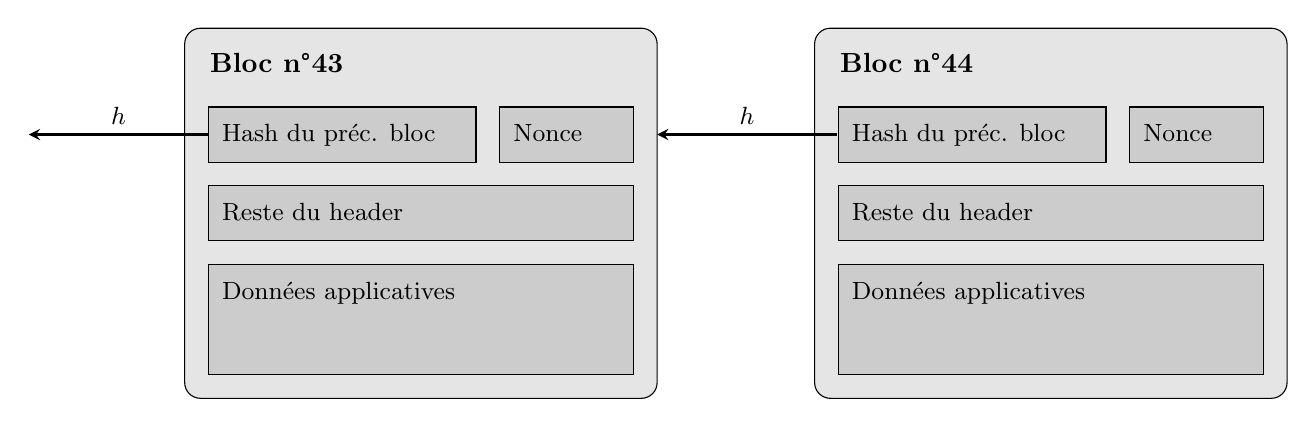
\begin{tikzpicture}[scale=1]
	\begin{scope}[shift={(3cm,-5cm)}, fill opacity=1]
		\bloc{0}{0}{Bloc n°43}
		\bloc{8}{0}{Bloc n°44}

		\fleche{6,3.35}{2.28, 0}{\small $\mathfrak{h}$}
		\fleche{-1.98,3.35}{2.28,0}{\small $\mathfrak{h}$}


		% Add more blocs as needed
	\end{scope}
\end{tikzpicture}
        \caption{Structure des blocs dans une Blockchain}
        \label{fig:blocs}
    \end{figure}


    \subsection{Preuve de travail}\label{subsec:pow}

    Pour rendre la création d'un bloc difficile, il existe plusieurs mécanismes.
    Le plus connu est la preuve de travail (PoW), mais il en existe d'autres,
    comme la preuve d'enjeu (PoS)~\cite{PoS}, ou la preuve de capacité
    (PoC)~\cite{PoC}. L'idée générale est de demander au créateur du bloc
    (appelé mineur) de résoudre un problème difficile. En revanche, la
    vérification de la solution doit être facile, pour que les autres
    participants puissent facilement vérifier la validité du bloc. Dans le cadre
    de mon stage, je me suis intéressé à la preuve de travail, qui est le
    mécanisme utilisé par Bitcoin.

    % Fonctionnement des preuves de travail
    La preuve de travail consiste à trouver à trouver un nonce (noté $c$), tel
    que :

    \begin{equation}
        \mathfrak{h}(c, h, d) < T
    \end{equation}

    Avec $\mathfrak{h}$ la fonction de hashage, $h$ le header du bloc (contenant
    le hash du bloc précédent), $d$ les données applicatives, et $T$ la target,
    définie par le protocole. Ainsi, il faudra tester tout les entiers $c$
    jusqu'à trouver un nonce qui vérifie cette équation. Plus $T$ sera petit,
    plus il sera difficile de trouver un tel $c$, inversement, plus $T$ sera
    grand, plus il sera facile de le trouver. On définit la difficulté comme
    l'inverse de la target $D = 1/T$.

    Afin de garantir que la création d'un bloc soit difficile, la difficulté est
    ajustée régulièrement. En effet, si le réseau au global augmente sa
    puissance de calcul, la difficulté de création d'un bloc risque de devenir
    trop faible et de permettre à un attaquant de créer des blocs plus vite que
    le reste du réseau. Pour éviter cela, la difficulté est ajustée par le
    protocole tous les 2016 blocs. Cet ajustement est paramétré de manière à ce
    que le temps moyen de création d'un bloc reste d'environ 10 minutes.

    % Les k derniers blocs de la chaîne sont instable
    Malgré ce mécanisme de preuve de travail, il est toujours possible que
    l'adversaire soit "chanceux" et trouve le nonce plus vite que les autres
    parties honnêtes du réseau. Cependant, statistiquement, il ne peut pas être
    "chanceux" à chaque fois. Le calcul de la probabilité de réussir à invalider
    un bloc à $k$ profondeur a été fait dans l'article de
    Nakamoto~\cite{bitcoin}, en modélisant le problème par un processus de
    Poisson :
    
    \begin{equation}
        1 - \sum_{i=0}^{k} \frac{\lambda^i e^{-\lambda}}{i!} (1-(q/p)^{k-i})
    \end{equation}

    Avec respectivement $q$ et $p$ les proportions de puissances de calcul de
    l'adversaire et de l'honnête (telle que $q + p = 1$) et $\lambda$ le taux de
    création de blocs ($\lambda = k(q/p)$). Ce calcul a permis d'estimer 
    qu'avec 1/3 de la puissance de calcul, l'adversaire a une probabilité de
    $P = 10^{-6}$ de réussir à invalider un bloc de profondeur 50.


\section{Le modèle statique}\label{sec:statique}

    Il existe un certain nombre de modèles pour décrire le fonctionnement des
    systèmes Blockchain. J'ai commencé par étudier un modèle
    statique~\cite{static_backbone} où la puissance de calcul de l'ensemble de
    nœud est fixée. Ce modèle est plus simple à étudier, mais reflétera moins la
    réalité qu'un modèle dynamique, où la puissance de calcul du réseau peut
    varier.
    

    \subsection{Présentation du modèle}\label{subsec:statique-presentation}

    Le modèle statique appréhende les systèmes Blockchain comme un ensemble de
    $n$ nœuds dont la puissance de calcul est fixée. Parmi ces $n$ nœuds, il y
    a $n-t$ nœuds honnêtes et $t$ nœuds malveillants. Les nœuds honnêtes suivent
    le protocole à la lettre, tandis que les malveillants peuvent tenter de le
    violer. Ce modèle se place dans une hypothèse synchrone, où le temps
    s'écoule en rondes. Par ailleurs, les canaux de communications sont
    considérés comme fiables, c'est à dire qu'il n'y a ni perte, ni altération
    ni duplication des messages émis. Ainsi, ces hypothèses assurent que tous
    les messages émis au cours d'une ronde sont reçus par leurs destinataires
    avant la fin de celle-ci. Qu'il soit malveillant ou honnête, chaque nœud ne
    peut faire qu'un nombre fixé $r$ requêtes par ronde à une fonction de
    hashage pour tenter de miner un bloc.

    \paragraph{Probabilité de réussite} On note $P_T$ la probabilité d'un unique
    nœud honnête de réussir à trouver un bloc en une seule requête à la fonction
    de hashage. On note $\kappa$ le nombre de bits de la sortie de la fonction
    de hashage. $T$ est la target utilisée pour la preuve de travail. Étant
    donnée que la fonction de hashage est indistinguable d'un processus
    uniforme, la probabilité de trouver un bloc en une seule requête est $P_T =
    T/2^\kappa$. On note $f$ la probabilité qu'au moins un nœud honnête trouve
    un bloc en une ronde. Cela revient à calculer l'espérance de la loi
    binomiale de paramètre $r$ et $P_T$, soit :

    \begin{equation}\label{eq:proba-bloc}
        f = 1 - (1 - P_T)^{r(n-t)}
    \end{equation}

    À partir de $f$, les auteurs introduisent trois variables aléatoires $X$,
    $Y$ et $Z$. $X_i = 1$ si au moins un nœud honnête trouve un bloc à la ronde
    $i$, $X_i = 0$ sinon. $Y_i = 1$ si exactement un nœud honnête trouve un bloc
    à la ronde $i$, $Y_i = 0$ sinon. $Z_i = 1$ si un nœud malveillant trouve un
    bloc à la ronde $i$, $Z_i = 0$ sinon. L'espérance et les variations de $X$,
    $Y$ et $Z$ sont facilement calculables puisqu'il s'agit de variables
    binomiales.

    \paragraph{Exécution typique} Le modèle introduit ensuite le concept
    d'exécution typique. Une exécution sera dite typique si les variables
    aléatoires $X$, $Y$ et $Z$ ne s'écartent pas trop de leur espérance, au plus
    d'un facteur $\varepsilon \in (0,1)$. Une exécution peut être dite typique
    uniquement si le nombre rondes considérées est suffisamment grand. On note ce
    paramètre $\Lambda \geq 2/f$. Pour finir, on partira du principe que la
    fonction de hashage est inviolable, c'est à dire qu'on omettra les cas de
    collisions. Les auteurs prouvent que la probabilité d'une exécution typique
    vaut $1 - e^{O(\varepsilon^2\Lambda f+\kappa-\log{L})}$, avec $L$ le nombre
    de rondes depuis le début du protocole.


    \subsection{Propriétés du modèle}\label{subsec:statique-proprietes}

    Avec ces outils, les auteurs du modèle ont pu prouver deux
    propriétés fondamentales du protocole Bitcoin si on reste dans le cadre
    d'une exécution typique. Ces deux propriétés sont le préfixe commun et la
    qualité de la chaîne. Le préfixe commun assure que les chaînes des nœuds
    honnêtes ont un préfixe commun important, tandis que la qualité de la chaîne
    assure que la proportion de blocs malveillants dans la chaîne des nœuds
    honnêtes est limitée.

    \paragraph{Préfixe commun} Le préfixe commun est garanti si la proportion de
    nœuds malveillants est inférieure à celle des nœuds honnêtes. Dans une
    exécution typique, si $t < n - t$, alors les chaînes des nœuds honnêtes ont
    un nombre de blocs $k$ à tronquer de la chaîne originale pour obtenir un
    préfixe commun qui est $k \geq 2\Lambda f$.

    \paragraph{Qualité de la chaîne} La qualité de la chaîne définit à quel
    point la chaîne des nœuds honnêtes est polluée par des blocs malveillants.
    La qualité de la chaîne sera idéale si la proportion de blocs appartenant
    aux malveillants est exactement égale à leur proportion de puissance de
    calcul. Les auteurs ont prouvé que dans une exécution typique, la qualité de
    la chaîne $t/n$ est garantie avec une probabilité écrasante si $t/n < 1/3$.

    
\section{Le modèle dynamique}\label{sec:dynamic}

    Dans un autre article~\cite{dynamic_backbone} les auteurs proposent une
    extension dynamique du modèle statique~\cite{static_backbone}. Ce modèle
    introduit la variation de la puissance de calcul du système au cours du
    temps. Il reprend les mêmes concepts que le modèle statique, mais rajoute un
    certain nombre d'outils mathématiques pour prendre en compte cette
    variation.


    \subsection{Présentation du modèle}\label{subsec:dynamic-presentation}

    La principale différence entre le modèle statique et le modèle dynamique est
    que le nombre de nœuds $n$ n'est plus fixé. Or, pour maintenir un rythme
    de création de blocs constant, le protocole doit ajuster la difficulté de
    création de blocs. Ainsi, si le nombre de nœuds augmente, la difficulté
    doit augmenter, inversement si le nombre de nœuds diminue. Donc la
    difficulté devient variable.

    \paragraph{Fonction de recalcul de la target} Pour ajuster la difficulté, le
    protocole doit recalculer la target $T$ tous les $J$ blocs ($J = 2016$ blocs
    dans le cas de Bitcoin). On nomme cet intervalle entre deux recalculs une
    \textit{epoch}. Les auteurs introduisent la fonction $D(\cdot)$ de recalcul
    de la difficulté. Cette fonction va être exécutée par chaque nœud à la fin
    de chaque epoch, pour définir la nouvelle target $T'$. La variation de la
    difficulté entre deux epochs est bornée par un facteur $\tau$ ($\tau = 4$
    dans le cas de Bitcoin). C'est à dire que $T/\tau \leq T' \leq T\cdot\tau$.
    Cela permet d'éviter des variations trop brutales de la difficulté, ce qu'un
    attaquant pourrait exploiter.

    \paragraph{Exécutions $(\eta, \theta)$-good} La fonction $D(\cdot)$ est
    exécutée par chaque nœud à la fin de chaque epoch. Sauf que chaque nœud ne
    dispose pas de la même information. En effet, le réseau subit un temps de
    propagation, et chaque nœud ne reçoit pas les mêmes blocs exactement au même
    moment. Il est donc légitime pour deux nœuds honnêtes de ne pas avoir
    exactement la même target $T$. Les auteurs introduisent donc le concept
    d'exécution $(\eta, \theta)$-good, qui assure que le taux de production des
    blocs honnêtes ne s'écartent pas trop du taux de production théorique
    attendu par le protocole. Une exécution sera dite $(\eta, \theta)$-good si :

    \begin{equation}
        \eta f \geq f(T, n) \geq \theta f
    \end{equation}

    Avec $f$ la nouvelle target calculée par le nœud, $T$ l'ancienne target,
    et $n$ le nombre de rondes considérées depuis la dernière epoch.

    \paragraph{Environnement $(\gamma, s)$-respecting} Un environnement sera 
    dit $(\gamma, s)$-respecting si la variation du nombre de nœuds est bornée
    d'un facteur $\gamma$ toutes les $s$ rondes. Cela assure que la variation
    du nombre de nœuds n'est pas trop brutale. En effet, il est raisonnable de
    supposer que dans la réalité, le nombre de nœuds ne varie pas trop vite.

    \paragraph{Variables aléatoires} Les auteurs modifient ensuite la définition
    des variables aléatoires $X$, $Y$ et $Z$ introduites dans le modèle
    statique. Avec une target dynamique, il ne suffit plus de considérer un bloc
    crée ou non, mais aussi de prendre en compte la target utilisée pour le
    créer. En effet, deux blocs créés avec des targets différentes n'ont pas la
    même probabilité d'être créés, ni la même importance lors de la comparaison
    entre deux chaînes. Les auteurs modifient donc les variables $X$, $Y$ et $Z$
    pour valoir $0$ si aucun bloc est créé, et $D$ si un bloc est créé avec une
    difficulté $D$.


    \subsection{Propriétés du modèle}\label{subsec:dynamic-resultats}

    À partir de ces nouveaux outils, les auteurs ont pu prouver deux autres
    propriétés importantes du protocole Bitcoin : la \textit{persistance} et la
    \textit{vivacité}. La \textit{persistance} assure qu'une donnée une fois
    inscrite dans la chaîne est immuable, tandis que la \textit{vivacité} assure
    qu'une donnée valide sera inscrite dans la chaîne.

    \paragraph{Persistance} La \textit{persistance} assure qu'une donnée une
    fois inscrite dans la chaîne est immuable. Dans une exécution typique, et un
    environnement $(\gamma, s)$-respecting, la \textit{persistance} est garantie
    quand la donnée est inscrite dans la chaîne à une profondeur $k$ telle que :

    \begin{equation}
        k \geq \frac{\theta \gamma J}{4\tau}
    \end{equation}

    \paragraph{Vivacité} La \textit{vivacité} assure qu'une donnée valide sera
    inscrite dans la chaîne. Les auteurs ont prouvé que dans une exécution
    typique, et un environnement $(\gamma, s)$-respecting, la \textit{vivacité}
    est garantie avec une probabilité écrasante en un temps fini.


\section{Algorithme de compression MLS}\label{sec:mls}
 
    Une Blockchain peut vite devenir très volumineuse. En effet, c'est une
    structure de données en ajout uniquement. Ainsi, aujourd'hui, la chaîne
    Bitcoin pèse plus de 450 Go après 15 ans d'existence. La chaîne Ethereum
    pèse quant à elle plus de 1 To après seulement 8 ans d'existence. De plus la
    croissance de telles chaînes est linéaire. Cela pose un problème d'accès à
    un tel réseau : si un nœud doit stocker l'intégralité de la chaîne, il lui
    faudra un espace de stockage important, et tous les appareils ne disposent
    pas d'un tel espace de stockage. C'est pourquoi il est important de trouver
    des solutions pour compresser la chaîne.
    
    Il existe aujourd'hui des solutions de compression et elles comportent
    toutes des compromis. J'ai étudié l'une d'entre elles, l'algorithme de
    compression \textit{Mining in Logarithmic Space} (MLS)~\cite{mls}. MLS est
    un algorithme de compression de la chaîne de bloc. L'article s'appuie sur
    les travaux du modèle statique~\cite{static_backbone}, c'est pourquoi il
    était important pour moi de travailler sur ce modèle avant de m'intéresser à
    MLS.
    

    \subsection{Présentation de l'algorithme}\label{subsec:mls_presentation}

    MLS fait partie de la famille des algorithmes NIPoPoWs (Non-Interactive
    Proofs of Proof of Work). Ces algorithmes permettent de prouver que les
    preuves de travail ont été effectuées sans avoir à effectivement posséder
    les blocs. L'algorithme MLS va échantillonner les blocs de la chaîne, et ne
    garder que les blocs les plus importants. Cependant, en échantillonnant les
    blocs, des données applicatives vont être perdues : on partira donc du
    principe que la chaîne que l'on va compresser effectue des snapshots de
    l'état applicatif à chaque bloc.
    
    Deux algorithmes seront nécessaires pour utiliser MLS : un algorithme de
    compression et un algorithme de comparaison, permettant de comparer deux
    compressés. Les deux algorithmes sont disponibles en annexe
    \ref{sec:mls_algo}.

    \paragraph{Niveau d'un bloc} Les auteurs introduisent le concept de niveau
    d'un bloc. Le niveau $\ell$ d'un bloc est défini comme le nombre de fois
    ou la target a été dépassée. Plus formellement :

    \begin{equation}
        \textrm{Le bloc } b \textrm{ est de niveau } \ell \Leftrightarrow
        \mathfrak{h}(b) \leq \frac{T}{2^\ell}
    \end{equation}

    Ainsi, un bloc de niveau $\ell$ est un bloc qui a dépassé la target de
    $2^\ell$ Étant donnée que la sortie de $\mathfrak{h}$ est uniforme, la
    probabilité qu'un bloc soit de niveau $\ell$ est $2^{-\ell}$. Donc tous les
    blocs seront de niveau 0, la moitié de niveau 1, le quart de niveau 2, etc.

    \paragraph{Algorithme de compression} L'algorithme MLS va échantillonner les
    blocs de la chaîne. Pour cela, il va d'abord chercher le niveau dit
    \textit{maximal} de la chaîne. Le niveau maximal est le niveau le plus haut
    qui possède au moins $2m$ bloc, $m$ étant un paramètre du système. On garde
    tous les blocs du niveau maximal. Ensuite, l'algorithme garde les $2m$
    derniers blocs de chaque niveau inférieur au niveau maximal, et les $m$
    derniers blocs du niveau supérieur.


    \paragraph{Chainage des blocs} Il est important de garder le bloc précédent
    dans la chaîne compressée pour pouvoir empêcher un adversaire de modifier un
    bloc au milieu de la chaîne. Cependant, comme l'algorithme ne garde pas tous
    les blocs, il est possible que le bloc précédent dans la chaîne initiale ne
    soit plus dans la chaîne compressée. Les auteurs propose de changer la
    structure de la Blockchain d'une liste simplement chaînée vers l'arrière à
    une liste à enjambement (\emph{skiplist}). Ainsi, chaque bloc contiendra le
    hash du dernier bloc de chaque niveau. On s'assure ainsi qu'on a toujours au
    moins une référence à un bloc qui sera contenu dans la chaîne compressée.

    \vspace{0.4cm}
    \begin{figure}[ht]
        \centering
        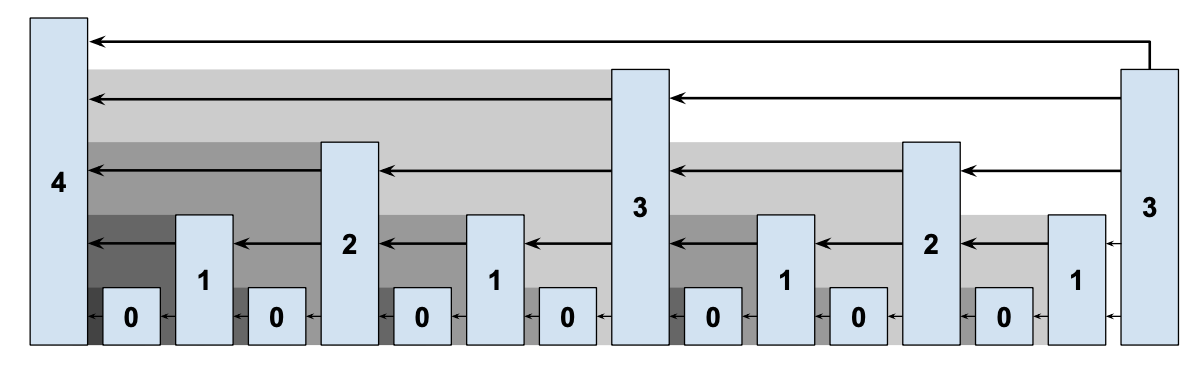
\includegraphics[width=0.8\textwidth]{figs/linking.png}
        \caption{Chainage des blocs dans MLS \cite{mls}}
        \label{fig:linking}
    \end{figure}

    
    \paragraph{Algorithme de comparaison} Les nœuds doivent être capables de
    comparer deux chaînes compressées pour choisir laquelle garder. L'algorithme
    de comparaison va chercher le dernier ancêtre commun de même niveau dans les
    deux compressés, et comparer les blocs à partir de ce point. Étant donné que
    l'algorithme de compression a gardé les blocs les plus \textit{rares}, le
    compressé ayant le plus de blocs de haut niveau sera celui qui témoigne
    d'une chaîne ayant demandé plus de travail avant la compression.


    \subsection{Propriétés de l'algorithme}\label{subsec:mls_proprietes}

    À l'aide des outils du modèle statique~\cite{static_backbone}, les auteurs
    ont pu prouver que l'algorithme MLS respecte trois propriétés importantes :
    la \textit{sécurité}, la \textit{concision} et l'\textit{idempotence}.
    
    \paragraph{Sécurité} La propriété de \textit{sécurité} assure que lors de la
    comparaison de deux chaînes compressées, l'algorithme de compression
    choisira le compressé honnête. Cette propriété a été prouvée dans le cas
    où l'adversaire possède moins d'un tiers du réseau, et que l'on est dans le
    cadre d'une exécution typique.

    \paragraph{Concision} La propriété de \textit{concision} assure que la
    taille de la chaîne compressée grandit de manière logarithmique par rapport
    à la chaîne originale $\mathcal{C}$ . Il a été prouvé que le compressé est
    de taille $2m \log{|\mathcal{C}|} + k$ avec $|\mathcal{C}|$ le nombre de
    blocs de la chaîne originale, $m$ le e paramètre de l'algorithme de
    compression, et $k$ les derniers blocs de la chaîne originale, que l'on ne
    compresse pas car ils sont instables.

    \paragraph{Idempotence} La propriété d'\textit{idempotence} assure que
    compresser une chaîne à laquelle on aurait préalablement ajouté un bloc est
    équivalent à compresser un compressé de cette chaîne à laquelle on aurait
    ajouté un bloc. Cette dernière propriété est importante pour garantir que
    l'on ne supprime pas des blocs dont on aurait besoin plus tard. La propriété
    d'\textit{idempotence} assure également que l'on puisse continuer de miner
    des blocs sur la chaîne compressée.
    

\section{MLS dans un modèle dynamique}\label{sec:mls_dynamic}


    L'algorithme de compression MLS~\cite{mls} a été conçu dans un modèle
    statique. Cependant, dans la réalité, le nombre de nœuds n'est pas fixé, et
    la difficulté de création de blocs doit être ajustée régulièrement. C'est
    pourquoi l'équipe de BC4SSI a travaillé sur une adaptation de l'algorithme
    de compression MLS à un modèle dynamique, plus proche de
    la réalité.

    La principale différence entre l'algorithme de compression MLS dans un
    modèle statique et un modèle dynamique est la variation de la difficulté.
    Cela a nécessité de modifier l'algorithme de compression et de comparaison
    pour prendre en compte cette variation (disponibles en annexe
    \ref{sec:mls_dyn_algo}). En effet, à présent, les difficultés des blocs sont
    prises en compte dans la comparaison des chaînes compressées.
    
    Les preuves ont aussi du être adaptées pour prendre en compte ce modèle
    dynamique. Ainsi, l'équipe a pu prouver qu'il était toujours impossible de
    supprimer un bloc de la chaîne compressée et que les propriétés de
    \textit{sécurité}, de \textit{concision} et d'\textit{idempotence} étaient
    toujours respectées dans la version dynamique de l'algorithme. Il a aussi
    été prouvé que la propriété du préfixe commun était toujours respectée en
    considérant les blocs du même niveau. C'est à dire que deux chaînes
    partagent un préfixe commun important de blocs de même niveau.

    \paragraph{Valeur de $m$} La valeur de $m$ est un paramètre important de
    l'algorithme de compression MLS. Il définit le nombre de blocs de chaque
    niveau que l'on garde dans la chaîne compressée. Choisi trop petit,
    l'adversaire risque de pouvoir créer une chaîne compressée plus difficile
    que la chaîne honnête par "chance". Choisi trop grand, la chaîne compressée
    deviendra trop volumineuse. Les auteurs de l'algorithme du modèle statique
    n'ont pas exprimé de valeur de $m$. Il s'agit pourtant d'un paramètre
    important pour utiliser l'algorithme dans la réalité. C'est pourquoi
    l'objectif de notre article est de proposer une valeur de $m$ pour
    l'algorithme de compression MLS dans un modèle dynamique. Ça sera l'objet de
    la suite de mon travail de recherche.
